\documentclass{article}
\renewcommand{\baselinestretch}{1.1}

% Language setting
% Replace `english' with e.g. `spanish' to change the document language
\usepackage['italiano']{babel}

% Set page size and margins
% Replace `letterpaper' with `a4paper' for UK/EU standard size
\usepackage[letterpaper,top=2cm,bottom=2cm,left=3cm,right=3cm,marginparwidth=1.75cm]{geometry}

% Useful packages
\usepackage{amsmath}
\usepackage{graphicx}
\usepackage[colorlinks=true, allcolors=blue]{hyperref}

\title{Caratteristica IV diodi al Silicio e Germanio}
\author{Benazzi Marco, Galante Sofia}

\begin{document}
\maketitle

\begin{abstract}
Nell'esperimento proposto è stata effettuta una misura della caratteristica IV di un diodo. Sui dati sperimentali è stato eseguito un fit rispetto l'equazione di Schockley per diodi ideali e si sono ottenuti come risultati per corrente inversa $I_0=(7.2 \pm 0.2)10^{-9} A$ e prodotto $ \eta V_T =(5 \pm 2)10^{-2}V$ per il diodo al Silicio, mentre $I_0=(2\pm1)10^{-5}A$ e $ \eta V_T=(7 \pm 1)10^{-2}V$ per quello al Germanio. 
\end{abstract}

\section{Introduzione}
Costruire le caratteristiche dei diodi del Germanio e del Silicio e confrontarli. A questo scopo dobbiamo misurare ciascun punto corrente-tensione da mettere nel piano I-V. Inoltre è utile calcolare i due valori di soglia per vedere come si comportano due semiconduttori diversi.

\section{Svolgimento dell'esperimento}
\subsection{Apparato Sperimentale}
\begin{itemize}
\item Alimentatore di bassa tensione modello: EB2025T TRIPLE OUTPUT PSU.
\item Multimetro digitale modello: FLUKE 77 IV.
\item Oscilloscopio modello: GOS-652G.
\item Potenziometro da 1K$\Omega$ composto da tre terminali.                        
\item Diodo p-n: AAZ15/OA47 Germanio, 1N914A/1N4446/1N4148 Silicio.
\item Scheda mille fori, utilizzata come base per realizzare il circuito, modello: GB3-243.
\item Cavi per la realizzazione del circuito e cacciavite per variare la tensione sul potenziometro.
\end{itemize}
\subsection{Realizzazione del circuito}
Prendendo il potenziometro si collega un terminale esterno con il ground e,  successivamente, si connette l’altro terminale esterno all’uscita più positiva dell’alimentatore a bassa tensione, in questo caso quella corrispondente a +5 Volt.
Il terminale centrale, invece, sarà collegato al puntale rosso del multimetro. L’altro puntale nero del multimetro si connette alla boccola del ground. Collegato a sua volta in un altro punto della piastra in cui sarà presente il ponte AB presente in Figura 1. Nella fase di calibrazione questo ponte sarà occupato da un cavo e successivamente dai diodi al germanio e al silicio.

\begin{figure}
\centering
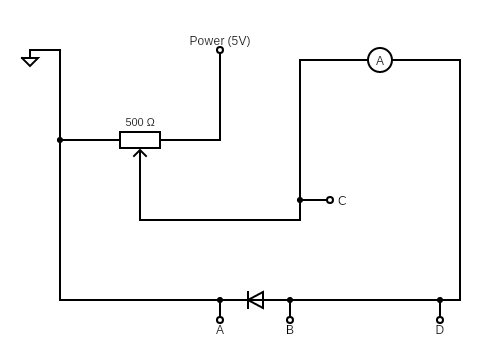
\includegraphics[scale=0.50]{Circuit.png}
\caption{Circuito utilizzato nell'esperimento e sottoposto a tensione iniziale di 5V} 
\end{figure}
\subsection{Calibrazione multimetro e oscilloscopio}
Questa fase è costituita dalla calibrazione degli strumenti che si ottiene confrontando la tensione misurata con l’oscilloscopio in funzione di quella misurata con il multimetro. Bisogna verificare quindi che tra le misure non ci sia uno scarto. Se gli strumenti sono calibrati otterremo, graficando le due tensioni, una retta inclinata di 45°. Se così non fosse invece avremo un offset e andranno modificati i valori di tensione presi con l’oscilloscopio in funzione di una successiva analisi dei dati.
A questo proposito si utilizza il circuito realizzato nella prima fase e rappresentato in Figura 1 e nel punto C si inserisce la sonda dell’oscilloscopio.
Si prendono circa 8 misure di tensioni (vedi tabella misure) che nel nostro caso sono comprese tra i 40 e i 210 milliVolt variando la tensione sul potenziometro. Per fare ciò si utilizza un cacciavite e si gira leggermente la vite sul potenziometro, così facendo stiamo variando il valore della resistenza. Avendo settato il multimetro su Volt possiamo leggere il valore della tensione che cambia sullo schermo.
\subsection{Misura di tensione dei diodi}
Per prima cosa bisogna la resistenza del potenziometro a 500 Ohm. Dopo aver spostato il potenziometro fuori dal circuito fissiamo il multimetro sulla resistenza e giriamo la vite del potenziometro finché non vediamo sullo schermo del multimetro il valore di 500 Ohm. Dopodichè possiamo posizionare nuovamente il potenziometro nella posizione iniziale.
Si sostituisce al cavo nel ponte AB il diodo ,al cui anodo colleghiamo la sonda dell’oscilloscopio (punto D, figura circuito) mentre  al catodo sarà collegato a massa.
Si prendono quindi circa 8 misure agendo sulla vite del potenziometro per variare la differenza di potenziale, misurata con l’oscilloscopio, e quindi la corrente misurata con il multimetro. 
Si procede utilizzando prima il diodo del silicio e in seguito quello del germanio.

\section{Analisi dati}
\subsection{Retta di calibrazione}
\begin{table}[h!]
\centering
 \begin{tabular}{||c|c||c|c|} 
 \hline
 ddp oscillosciopio(mV) & Incertezza(mV) & ddp multimetro (mV) & incertezza (mv) \\ [0.5ex]
 \hline\hline
 40 & 4.18 & 31.9 & 0.01 \\
 48 & 2.46 & 40.0 & 0.01 \\
 68 & 2.86 & 59.9 & 0.01 \\
 88 & 3.31 & 79.3 & 0.01 \\
 108 & 3.81 & 100.1 & 0.01 \\
 130 & 6.34 & 120.7 & 0.01 \\
 150 & 10.97 & 140.5 & 0.01 \\
 170 & 7.14 & 160.0 & 0.01 \\
 190 & 7.58 & 180.2 & 0.01 \\
 210 & 8.04 & 200.1 & 0.01 \\
\hline
 \end{tabular}
\caption{Punti sperimentali della tensione misurata dall'oscilloscopio}
\end{table}

\begin{figure}
\centering
\includegraphics[scale=0.15]{calib.png}
\caption{Retta di calibrazione per misure di tensione di oscilloscopio e multimetro} 
\end{figure}
Il fit effettuato tramite ROOT ha riportato un valore pari a \(m=(1.01\pm0.03)mV\) per il coefficiente angolare, consistente ad un fattore moltiplicativo unitario. L’irtercetta della retta, invece, presenta una discrepanza dall’orgine pari a \(q=(7\pm3)mV\), perciò nelle misure successive di tensione sui diodi è stato propagato linearmente l’errore dovuto all’offset della retta di calibrazione secondo l’equazione seguente:
\begin{equation}
V = (V_o - q)\pm(\sigma_o+\Delta q)
\end{equation}

Dove \(V_o\) è la ddp misurata dall’oscilloscopio, q l’offset della retta di calibrazione, \(\sigma_o\) e \(\Delta q\) gli errori associati. In paricolare, l’errore sulle misure effettuate tramite l’oscilloscopio è stato ottenuto tramite una propagazione in quadratura dell’errore del costruttore, quello sulla lettura e quello sulla misura dello zero.

\begin{equation}
\sigma_o = \sqrt{\sigma_c^2+\sigma_l^2+\sigma_z^2}
\end{equation}
\subsection{Caratteristica IV diodo al Silicio}
Di seguito sono riportati in tabella le misure di tensione e intensità di corrente restituite rispettivamente da oscilloscopio e multimetro; le misure sull’oscilloscopio tengono conto dell’offset della retta di calibrazione.
\begin{table}[h!]
    \centering
    \begin{tabular}{|||c|c||c|c||}
    \hline
    Intensità corrente (mA) & errore (mA) & Tensione diodo (mV) & errore (mV) \\
    \hline\hline
    0.10 & 0.01 & 520 & 46 \\
    0.21 & 0.01 & 560 & 46 \\
    0.41 & 0.01 & 600 & 47 \\
    1.03 & 0.01 & 640 & 47 \\
    2.22 & 0.01 & 680 & 48 \\
    4.29 & 0.01 & 720 & 48 \\
    8.46 & 0.01 & 760 & 49 \\
    14.84 & 0.01 & 800 & 49 \\
    \hline
    \end{tabular}
    \caption{Punti sperimentali di intensità corrente elttrica e tensione ai capi del diodo}
    \label{tab:my_label}
\end{table}
Il corrispondente grafico è stato riportato in scala semilogaritmica ed è stato eseguito un fit attraverso l’eqauzione caratteristica di un diodo ideale, o equazione di Schockely. In questa equazione compare \(I_0\) corrente inversa di saturazione del diodo, dipendente dalle caratteristiche interne al diodo e parametro di cui vogliamo effettuare una stima. \(V_D\) differenza di potenziale ai capi del diodo, \(\eta\) parametro adimensionale dipendente dalla geometria interna del cristallo (circa 2 per il silicio) e \(V_T\) corrispondente della temperatura in Volt, di valore atteso 0.026V per temperature intorno ai 300K.
\begin{equation}
I = I_0 [exp({\frac{V_D}{\eta V_T}})-1]
\end{equation}
\begin{figure}
    \centering
    \includegraphics[scale=0.19]{canvas.png}
    \caption{Caratteristica IV di un diodo al Silicio in scala semilogaritmica}
    \label{fig:my_label}
\end{figure}
Dal fit abbiamo potuto riscontrare una stima della corrente inversa del diodo \(I_0 = (7.2\pm0.2)10^{-6}mA\) e un valore per il prodotto \(\eta V_T=(5\pm1)10mV\). Si nota, inoltre, come i dati sperimentali seguano l’equazione modello utilizzata per il fit anche se il valore di chiquadro ridotto che si è ottenuto è inferiore a 1 di due ordini di grandezza, ciò suppioniamo a causa di una sovrastima degli errori per l’oscilloscopio.
\subsection{Caratteristica IV diodo al Germanio}
In modo analogo al caso precedente, abbiamo misurato la caratteristica IV di un diodo al Germanio. Di seguito sono riportati i punti sperimentali utilizzati per effettuare il fit tramite ROOT, con equazione modello (3). Dal fit abbiamo ottenuto un grafico della caratteristica IV che presentava un parametro di ampiezza \(I_0 =0.02+/-0.01 mA\) e un prodotto \(\eta V_T=(7+/-1)10mV\). Rispetto al caso precedente il test del Chiquadro fornisce un valore più attendibile ma comunque inferiore a 1 almeno di un ordine di grandezza.
\begin{table}[]
    \centering
    \begin{tabular}{||c|c|c|c||}
    \hline
    Intensità corrente (mA) & errore (mA) & Tensione diodo (mV) & errore (mV) \\
    \hline\hline
    0.10 & 0.01 & 120 & 23 \\
    0.12 & 0.01 & 160 & 43 \\
    0.27 & 0.01 & 200 & 43 \\
    0.56 & 0.01 & 240 & 43 \\
    1.00 & 0.01 & 280 & 24 \\
    1.33 & 0.01 & 300 & 24 \\
    1.77 & 0.01 & 320 & 24 \\
    2.45 & 0.01 & 340 & 23 \\
    3.25 & 0.01 & 360 & 25 \\
    4.32 & 0.01 & 380 & 25 \\
    5.62 & 0.01 & 400 & 25 \\
    \hline
    \end{tabular}
    \caption{Punti sperimentali di intensità di corrente elettrica e tensione ai capi del diodo}
    \label{tab:my_label}
\end{table}
\quad
\begin{figure}
    \centering
    \includegraphics[scale=0.20]{canvas2.png}
    \caption{caratteristica IV di un diodo al Germanio}
    \label{fig:my_label}
\end{figure}
\section{Conclusione}
Dall’esperimento realizzato si sono potute misurare la corrente inversa dei diodi e quello dato dal prodotto tra il parametro  \(\eta\) e il corrispondente della temperatura in Volt \(V_T\). I valori ottenuti per il diodo al Silicio sono: \(I_0=(7.2 \pm 0.2)10^{-9}A\) e prodotto \(\eta V_T =(5 \pm 2)10^{-2}V\) per il diodo al Silicio, mentre \(I_0=(2\pm1)10^{-5}A\) e \(\eta V_T=(7 \pm 1)10^{-2}V\) per quello al Germanio. 

\end{document}
\bibliographystyle{alpha}
\bibliography{sample}
